\documentclass{article}
\usepackage{graphicx}
\usepackage{tabularx}
\usepackage{float}
\usepackage[width=18cm, height = 25cm]{geometry}

\title{Work report 140222: Co-sputtered ZnO-SnO$_2$}
\author{Rob Treharne}

\begin{document}

\maketitle

\section{Overview}

Samples for Binghampton. Co-sputtered ZTO films on conductive substrates.

Note that the composition profile now runs diagonally from bottom left to top left instead of horizontally from left to fight. This is because the SnO2 target was removed and re-installed for use with a different magnetron.


\section{Samples}

\begin{table}[h!]
\caption{Sample deposition parameters. Film deposited on 1mm thick aluminaborosilicate glass (ABS) substrates coated with a $250$ nm thick film of ITO ($10$ $\Omega/$square).}
\centering
\begin{tabular}{l|c}
\hline\hline
 ID & 140519\_3  \\
\hline
Material & ZnO:SnO$_2$  \\
RF power (W) & 70:109 \\
Ar pressure (mTorr) & 5  \\
dep. time (min) & 30 \\
T$_{dep}$ ($^{\circ}$C) & 18  \\
\hline
\end{tabular}
\end{table}




\section{Film profiles}

\begin{figure}[ht]
\centering
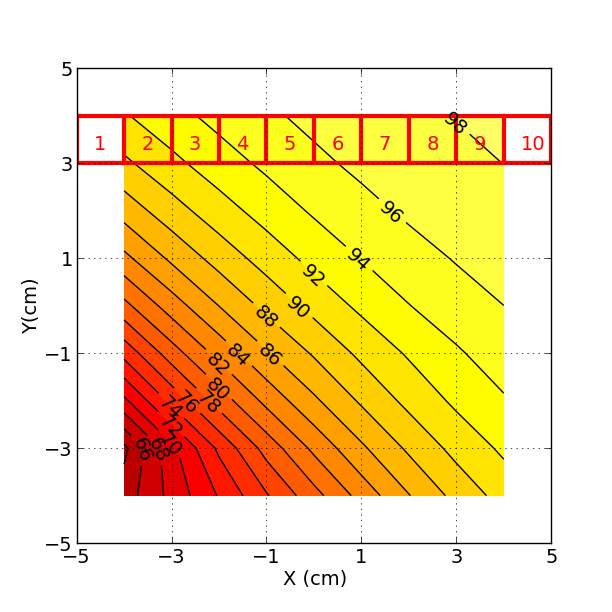
\includegraphics[width=0.5\textwidth]{140519_3_ZnO_SnO2_pieces_70-109.png}
\caption{\label{fig:3} 140519\_2\_ZnO\_SnO$_2$: $\%$ wt. SnO$_2$ profile of co-sputtered film. Red sample series cut from sample.}
\end{figure}



\begin{table}[p]
\caption{Aporoximate $\%$ wt. SnO$_2$ content series cut from ZTO samples.}
% title of Table
\centering
% used for centering table
\begin{tabular}{c c }
% centered columns (4 columns)
\hline\hline
%inserts double horizontal lines
Piece & Red Series  \\ [0.5ex]
% inserts table
%heading
\hline
% inserts single horizontal line
1 & 89.9  \\
2 & 91.6   \\
3 & 93.1  \\
4 & 94.4   \\
5 & 95.5  \\
6 & 96.4   \\
7 & 97.1   \\
8 & 97.7   \\
9 & 98.0  \\
10 & 98.1   \\
% [1ex] adds vertical space
\hline
%inserts single line
\end{tabular}
\label{table:nonlin}
% is used to refer this table in the text
\end{table}






\end{document}